%LTeX: language=pt-br
% !TeX root = Apostila_IM381.tex

\cleardoublepage
\section{Solução aproximada de problema unidimensional - barra}

    Conforme mostrada na seção anterior, a equação diferencial da barra é dada pela equação:

    \begin{equation}
        E A \frac{d^2u}{dx^2} = -p(x),
    \end{equation}

    \noindent já considerando $E$, $A$ constantes.
    
    Nesta seção, vamos resolver esta equação de forma numérica. Dada a simplicidade desta equação, é possível avaliar a qualidade de nossa aproximação comparando-a com a solução analítica. Porém, de forma geral, não teremos uma solução de referência para avaliar nossa aproximação.

    O procedimento apresentado aqui é discutido para o caso específico da barra, porém ele pode ser usado para qualquer equação diferencial, ordinárias ou parciais. Na Seção \ref{sec:conducao}, ele será usado para o problema de condução de calor. Na Seção \ref{sec:estado_plano}, será usado no equilíbrio de estruturas elásticas.

    \subsection{Forma forte e forma fraca}

        Para exemplificar, resolveremos a seguinte equação diferencial com as seguintes condições de contorno (Figura \ref{fig:barra_exemplo_deducao}):

        \begin{figure}[h!]
            \centering
            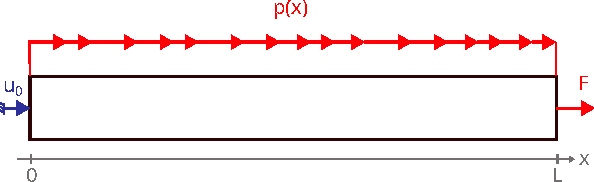
\includegraphics[scale=1]{Figures/2-Resmat/Barra_exemplo.pdf}
            \caption{Barra que servirá de exemplo.}
            \label{fig:barra_exemplo_deducao}
        \end{figure}

        \begin{equation}
            \begin{array}{c}
                E A \frac{d^2u}{dx^2} = -p(x)\\
                u(0) = u_0\\
                N_x(L) = \left.EA\frac{du}{dx}\right|_{x=L} = F
            \end{array}
        \end{equation}

        Embora analisemos este caso específico como um exemplo, o procedimento matemático é o mesmo para qualquer combinação de condições de contorno.

        A equação diferencial em sua forma original é chamada \textbf{forma forte}. Esta é a equação que obtemos diretamente das condições de equilíbrio do sistema ou de balanços de energia.

        A solução $u(x)$ dessa equação diferencial deve pertencer ao espaço de Sobolev $\mathcal{H}^1$ (Seção \ref{sec:algelin}). Mais especificamente, consideraremos aqui que a solução pertence ao espaço das funções com todas as derivadas contínuas (funções suaves) $C^\infty \subset \mathcal{H}^1$, e isso acontecerá se os esforços aplicados forem desta forma também.

        Portanto, definimos um espaço chamado espaço das funções teste $V$ (\textit{test functions}), que contém as soluções candidatas desta equação diferencial (incluindo sua solução):

        \begin{equation}
            V = \left\{u| u \in \mathcal{H}^1, u(0)=u_0 \right\}
        \end{equation}

        Na verdade, o espaço $V$ não é tecnicamente um espaço vetorial, pois ela não respeita o princípio da linearidade. Isto é, dadas duas funções $u_1,u_2 \in V$, $u_1(0) + u_2(0) \neq u_0$, logo, $u_1(x) + u_2(x) \notin V$. Entretanto, se pegarmos apenas os termos com $x \neq 0$ de cada função, ela se comportará como um espaço vetorial. Portanto, daqui em diante, trataremos ela como se fosse um espaço vetorial.

        Definiremos também um outro espaço, bastante similar, chamado espaço das funções peso $W$ (\textit{trial functions}). A diferença entre eles é que esté é realmente um espaço vetorial, com o(s) ponto(s) de condição de contorno de Dirichlet nulos:

        \begin{equation}
            W = \left\{w| w \in \mathcal{H}^1, w(0)=0 \right\}
        \end{equation}

        Podemos, então reescrever a equação diferencial da seguinte forma. Se a equação diferencial deve se anular, então o produto interno entre ela e uma função peso $w(x)$ também deve se anular, para qualquer $w(x) \in W$:

        \begin{equation}
            \int_0^L w(x)\left(EA\frac{d^2u}{dx^2} + p(x)\right) dx= 0 , \quad \forall w(x) \in W
        \end{equation}

        Suprimiremos a dependência de $x$ nas equações para simplificar a notação, porém ela permanece.

        Esta expressão é similar ao que se estuda na mecânica como o princípio do trabalho virtual. Este princípio enuncia que, dados os esforços externos e internos que mantenham o sistema em equilíbrio, se calcularmos o trabalho desses para qualquer campo de deslocamento (que obedeçam às restrições cinemáticas do problema), este deve ser nulo. Isto é, o trabalho das forças reais, quando sujeitas a um deslocamento virtual qualquer, deve ser nulo.

        Podemos reescrever a expressão acima, utilizando o procedimento de integração por partes:


        \begin{equation}
            \int_0^L EA w \frac{d^2u}{dx^2} dx + \int_0^Lwp(x) dx = 0
        \end{equation}

        \begin{equation}
            -\int_0^L EA \frac{dw}{dx} \frac{du}{dx} dx  + \left[EA w \frac{du}{dx}\right]_0^L+ \int_0^Lwp(x) dx = 0
        \end{equation}

        \begin{equation}
            \int_0^L EA \frac{dw}{dx} \frac{du}{dx} dx  = F w(L) + \int_0^Lwp(x) dx , \quad \forall w(x) \in W
            \label{eq:forma_fraca}
        \end{equation}

        Esta expressão é chamada \textbf{forma fraca}. As formas fraca e forte são equivalentes, mesmo que os nomes induzam o leitor a achar que uma delas se sobressaia a outra de alguma forma. Ambas descrevem de forma única a equação diferencial, e existe apenas uma única solução para ambas. Na forma fraca, entretanto, essa unicidade de solução só é garantida pelo fato da função peso poder assumir qualquer função em $W$.

        Na forma fraca, as condições de contorno de Dirichlet ainda devem aparecer explicitamente na definição de $u(x)$, entretanto, as condições de Neumann aparecem implicitamente nos termos de contorno que aparecem da integração por partes.

        Muitas vezes, podemos encontrar a forma fraca representada a partir de operadores bidirecionais, isto é:

        \begin{equation}
            a(w,u)  = (w,p)
        \end{equation}

        \noindent no qual $a(w,u)$ é um operador comutativo, que representa a integral à esquerda da igualdade. Já o termo $(w,p)$ representa os termos de esforços que aparecem do lado direito da igualdade.

        \subsubsection*{Equivalência entre as formas forte e fraca}

        Conforme dito na seção anterior, as formas fraca e forte são equivalentes, e encontrar a solução que satisfaça uma é equivalente a encontrar a solução da outra. A prova de que a solução da forma forte é solução da forma fraca já foi demonstrada na seção anterior, através da integração por partes. Agora, nos preocupamos em fazer o caminho inverso, provar que a solução da forma fraca implica na solução da forma forte.

        Suponha que $u(x)$ seja solução da forma fraca. Logo $u(0) = u_0$ ($w(0) = 0$) e:

        \begin{equation*}
            \int_0^L EA \frac{dw}{dx} \frac{du}{dx} dx  = F w(L) + \int_0^Lwp(x) dx , \quad \forall w(x) \in W
        \end{equation*}

        Aplicando integração por partes:

        \begin{equation*}
            -\int_0^L EA w \frac{d^2u}{dx^2} dx +  \left[EA w \frac{du}{dx}\right]_0^L = F w(L) + \int_0^Lwp(x) dx , \quad \forall w(x) \in W
        \end{equation*}

        \begin{equation*}
            \int_0^L EA w(x) \left(\frac{d^2u}{dx^2} + p(x)\right) dx +  w(L)\left[F - EAu'(L) \right] = 0 , \quad \forall w(x) \in W
            \label{eq:fraca_igual_forte}
        \end{equation*}

        Para que esta igualdade se verifique, basta que:

        \begin{equation*}
            I = \frac{d^2u}{dx^2} + p(x) = 0
        \end{equation*}

        \begin{equation*}
            II = F - EA u'(L) = 0
        \end{equation*}

        Como a forma fraca é válida para qualquer $w(x) \in W$, então podemos verificar para um exemplo de $w(x)$:

        \begin{equation*}
            w(x) = \phi(x)\left(\frac{d^2u}{dx^2} + p(x)\right)
        \end{equation*}

        \noindent no qual $\phi(x)$ é uma função suave no intervalo $(0,L)$ e satisfaz $\phi(0) = \phi(L) = 0$. Por exemplo, se $\phi(x) = x(L-x)$, então $w(0) = 0$, logo $w(x) \in W$. Inserindo este valor na Eq. \eqref{eq:fraca_igual_forte}:

        \begin{equation*}
            \int_0^L EA \phi\left(\frac{d^2u}{dx^2} + p(x)\right)^2 dx + 0 = 0
        \end{equation*}

        Como $\phi(x) >0$ e $\left(\frac{d^2u}{dx^2} + p(x)\right)^2 \geq 0$ para qualquer $x$ entre $0$ e $L$, então para que a integral se anule, $\frac{d^2u}{dx^2} + p(x) = 0$ para todo $x$ entre $0$ e $L$.

        Agora que provamos que $I=0$, a Eq. \eqref{eq:fraca_igual_forte} pode ser reduzida a:

        \begin{equation*}
           w(L)\left[F - EAu'(L) \right] = 0 , \quad \forall w(x) \in W
        \end{equation*}

        Como $W$ não impõe nenhuma restrição no valor de $w(L)$, então este ainda pode assumir qualquer valor. Portanto, a única forma dessa igualdade ser verificada é se:

        \begin{equation*}
            F - EAu'(L) = 0 
        \end{equation*}

        Portanto, $II = 0$ é verificado. Desta forma, com as expressões de $I$, $II$ e da condição de Dirichlet imposta em $V$, temos que a solução da forma fraca também é solução da forma forte.



    \subsection{Método dos Resíduos Ponderados e Método de Galerkin}

        Até o momento, trabalhamos apenas com soluções exatas da equação diferencial. Salvo casos muito específicos, normalmente não será viável ou possível resolver o problema desta forma. Portanto, propomos aqui um método para aproximar a solução.

        Suponha que agora, desejamos obter uma solução aproximada $u^h(x)$ da equação diferencial. Esta solução pertencerá a um espaço $V^h$. Isto é:

        \begin{equation}
            u^h(x) \in V^h \subset V
        \end{equation}

        O espaço original $V$ possui dimensão infinita. Definimos o subespaço $V^h$ tal que este possua dimensão finita.

        Similarmente, definimos uma função peso $w^h(x) \in W^h \subset W$.

        O \textbf{Método dos Resíduos Ponderados} implica em obter a função $u^h(x)$ que zere o resíduo de seu produto interno com qualquer $w^h(x),$ isto é:

        \begin{equation}
            \int_0^L w^h(x)\left(EA\frac{d^2u^h}{dx^2} + p(x)\right) dx= r = 0 , \quad \forall w^h(x) \in W^h
        \end{equation}

        Em um procedimento similar ao anterior, obtemos a equação na forma:

        \begin{equation}
            \int_0^L EA \frac{dw^h}{dx} \frac{du^h}{dx} dx  = N_x(L) w^h(L) - N_x(0) w^h(0) + \int_0^Lw^hp(x) dx , \quad \forall w^h(x) \in W
        \end{equation}

        Antes de prosseguir, vamos fazer algumas considerações sobre as fontes de erro na aproximação da nossa solução. Primeiramente, por se tratar de um subespaço, a solução aproximada será a mais próxima possível da projeção da solução real neste mesmo subespaço (análogo à projeção de vetores, Figura \ref{fig:projecao}). Entretanto, ainda haverá erros devido aos termos fora do subespaço de aproximação.

        \begin{figure}[h!]
            \centering
            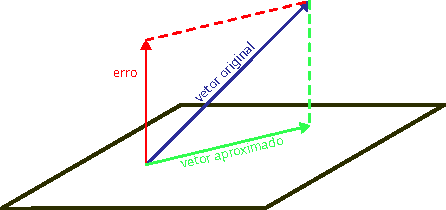
\includegraphics[scale=1]{Figures/3-Barra/Projecao.pdf}
            \caption{Exemplo de projeção de vetor em um subespaço: projeção de um vetor de $\mathbb{R}^3$ em $\mathbb{R}^2$}
            \label{fig:projecao}
        \end{figure}

        Sobre as condições de contorno, as condições de Dirichlet continuam sendo aplicadas explicitamente em $u^h(x)$, portanto, elas continuam exatas. Entretanto, as condições de Neumann aparecem implicitamente nos termos da integração por partes. Isto é, as condições de Neumann também podem não ser exatas.

        A forma mais usual, no contexto de elementos finitos, para continuar a solução dessa equação é utilizando o \textbf{Método de Galerkin}. Para este, assumimos que os subespaços $V^h$ e $W^h$ são iguais (salvo o termo de condição de contorno). Isto é $V^h = W^h$.

    \subsection{Funções de forma}

        Como os espaços $V^h$ e $W^h$ são finitos, podemos escrever qualquer termo deles como uma combinação linear de uma base que forme este espaço. Chamaremos estas funções que formam uma base desse espaço \textbf{funções de forma}, $N_1(x), N_2(x), \cdots, N_n(x)$. Portanto, podemos escrever o deslocamento e a função peso como:

        \begin{equation}
            u^h(x) = a_1 N_1(x) + a_2 N_2(x) + \cdots + a_n N_n(x) = \sum_{i=1}^n a_i N_i(x) =
            \begin{bmatrix}
                N_1 & 
                N_2 &
                \cdots&
                N_n
            \end{bmatrix}
            \begin{Bmatrix}
                a_1 \\ 
                a_2 \\
                \vdots\\
                a_n
            \end{Bmatrix} 
            = \mathbf{N} \mathbf{a}
        \end{equation}

        \begin{equation}
            w^h(x) = b_1 N_1(x) + b_2 N_2(x) + \cdots + b_n N_n(x) = \sum_{i=1}^n b_i N_i(x) = \mathbf{N} \mathbf{b}
        \end{equation}

        Substituíndo essas expressões na forma fraca:

        \begin{equation*}
            \int_0^L EA \left(\sum_{i=1}^n b_i\frac{dN_i}{dx}\right) \left(\sum_{j=1}^n a_j\frac{dN_j}{dx}\right) dx = \left(\sum_{i=1}^n b_i N_i(L)\right)F + \int_0^L \left(\sum_{i=1}^n b_i N_i(x)\right) p(x) dx
        \end{equation*}

        \begin{equation*}
            \sum_{i=1}^n b_i \left( \sum_{j=1}^n a_j\int_0^L EA \frac{dN_i}{dx} \frac{dN_j}{dx} dx \right) = \sum_{i=1}^n b_i \left(N_i(L) F + \int_0^L N_i(x) p(x) dx\right)
        \end{equation*}

        Como a equação deve se satisfazer para qualquer $w^h(x)$, então ela deve se satisfazer para qualquer combinação de $b_i$. Portanto, igualamos os termos com mesmo $b_i$ para obtermos um sistema de $n$ equações:

        \begin{equation*}
            \sum_{j=1}^n \left(\int_0^L EA \frac{dN_i}{dx} \frac{dN_j}{dx} dx\right) a_j = N_i(L) F + \int_0^L N_i(x) p(x) dx, \quad i=1,2\cdots, n
        \end{equation*}

        Este procedimento normalmente é representado em equação matricial, ficando da seguinte forma:

        \begin{equation*}
            \left(\int_0^L 
            \begin{Bmatrix}
            \frac{dN_1}{dx}\\
            \frac{dN_2}{dx}\\
            \vdots\\
            \frac{dN_n}{dx}\\
            \end{Bmatrix}
            EA
            \begin{bmatrix}
            \frac{dN_1}{dx} &
            \frac{dN_2}{dx} &
            \cdots &
            \frac{dN_n}{dx}
            \end{bmatrix} dx\right) \begin{Bmatrix}
            a_1\\
            a_2\\
            \vdots\\
            a_n\\
            \end{Bmatrix} = \mathbf{N}^T(L) F + \int_0^L \mathbf{N}^T p(x) dx
        \end{equation*}

        \begin{equation*}
            \left(\int_0^L 
            \mathbf{B}^T
            \mathbf{D}
            \mathbf{B} dx \right)
            \mathbf{a} = \mathbf{N}^T(L) F + \int_0^L \mathbf{N}^T p(x) dx
        \end{equation*}


        Chega-se portanto a um sistema linear. A matriz que aparece à esquerda é chamada \textbf{matriz de rigidez}:

        \begin{equation}
            \mathbf{K} = \int_0^1 
            \mathbf{B}^T
            \mathbf{D}
            \mathbf{B} dx = 
            \begin{bmatrix}
                K_{11} & K_{12} & \cdots & K_{1n}\\
                K_{21} & K_{22} & \cdots & K_{2n}\\
                \vdots & \vdots & \ddots & \vdots\\
                K_{n1} & K_{n2} & \cdots & K_{nn}\\
            \end{bmatrix}
        \end{equation}

        Esta matriz é uma matriz quadrada, simétrica e semi-positivo definida. Ela normalmente é escrita como um produto entre uma matriz $\mathbf{B}$ e uma matriz $\mathbf{D}$. Estes representam, respectivamente, as relações cinemáticas e as propriedades do modelo de material usados no problema. De forma geral, para qualquer caso podemos escrever a matriz desta forma, variando esses termos de acordo com a física e o material.

        Do lado direito da igualdade, aparece o \textbf{vetor de forças nodais}:

        \begin{equation}
            \mathbf{f} = \mathbf{N}^T(1) F + \int_0^1 \mathbf{N}^T p(x) dx =
            \begin{Bmatrix}
                F_1\\
                F_2\\
                \vdots\\
                F_n
            \end{Bmatrix}
        \end{equation}

        Finalmente, as incógnitas do problema estão no vetor de \textbf{deslocamentos nodais}:

        \begin{equation*}
            \mathbf{a} =
            \begin{Bmatrix}
                a_1\\
                a_2\\
                \vdots\\
                a_n
            \end{Bmatrix}
        \end{equation*}

        Portanto, reduzimos o problema a um sistema linear:

        \begin{equation}
            \mathbf{K} \mathbf{a} = \mathbf{f} 
        \end{equation}

        Resolvendo este, obtemos os coeficientes $a_i$ e, portanto o campo de deslocamento aproximado $u^h(x)$.
    
    \subsection{Considerações sobre condições de contorno e a solução}
    \label{sec:condicao_contorno}

        Para aplicar as condições de contorno no sistema, normalmente já partimos do sistema montado.

        Para as condições de Neumann, isto é, condições na derivada do deslocamento, elas já aparecem do lado direito da expressão da forma fraca. No caso da barra, surge, por exemplo, no termo:

        \begin{equation}
            \mathbf{N}^T(1) F
        \end{equation}

        Portanto, deve-se avaliar todas as funções de forma no ponto de aplicação da força concentrada, que por sua vez, retorna um vetor:

        \begin{equation}
            \mathbf{N}^T(1) F = \begin{Bmatrix}
                N_1(1)\\
                N_2(1)\\
                \vdots\\
                N_n(1)
            \end{Bmatrix}
            F
        \end{equation}

        Este vetor é somado ao vetor de forças $\mathbf{f}$. Como veremos na próxima seção, em alguns pontos do domínio, chamados \textbf{nós}, todas as funções de forma são nulas, exceto uma, que assume valor unitário. Portanto, uma força aplicada neste nó aparece como:

        \begin{equation}
            \mathbf{N}^T(1) F = \begin{Bmatrix}
                0\\
                0\\
                \vdots\\
                F
            \end{Bmatrix}
        \end{equation}

        Para as condições de Dirichlet, temos que o deslocamento em algum ponto será dado, portanto:

        \begin{equation*}
            u(0) = u_0
        \end{equation*}

        \begin{equation*}
             \begin{bmatrix}
                N_1(0) & 
                N_2(0) &
                \cdots&
                N_n(0)
            \end{bmatrix}
            \begin{Bmatrix}
                a_1 \\ 
                a_2 \\
                \vdots\\
                a_n
            \end{Bmatrix}  = u_0
        \end{equation*}

        Novamente, essas condições de contorno devem ser aplicadas usualmente em nós, nos quais apenas uma função de forma será não nula, portanto, assumindo que $N_1(0) = 1$ e os outros nulos:

        \begin{equation*}
            a_1 = u_0
        \end{equation*}

        O sistema global, portanto, fica:

        \begin{equation*}
             \begin{bmatrix}
                K_{11} & K_{12} & \cdots & K_{1n}\\
                K_{21} & K_{22} & \cdots & K_{2n}\\
                \vdots & \vdots & \ddots & \vdots\\
                K_{n1} & K_{n2} & \cdots & K_{nn}\\
            \end{bmatrix}
            \begin{Bmatrix}
                u_0 \\ 
                a_2 \\
                \vdots\\
                a_n
            \end{Bmatrix}
            =
             \begin{Bmatrix}
                F_1 + R\\
                F_2\\
                \vdots\\
                F_n
            \end{Bmatrix}
        \end{equation*}

        \noindent no qual aparece uma reação de apoio $R$ na mesma linha (seguindo a lógica da condição de Neumann acima, porém em x = 0).

        A primeira linha desse sistema envolve uma incógnita a mais ($R$), portanto, podemos removê-la. Se quisermos calcular $R$ após resolver o sistema, basta voltarmos a esta linha:

        \begin{equation*}
            K_{11}u_0  + K_{12}a_2 + \cdots + K_{1n}a_n = F_1 + R
        \end{equation*}

        \begin{equation*}
            \begin{bmatrix}
                K_{21} & K_{22} & \cdots & K_{2n}\\
                \vdots & \vdots & \ddots & \vdots\\
                K_{n1} & K_{n2} & \cdots & K_{nn}\\
            \end{bmatrix}
            \begin{Bmatrix}
                u_0\\
                a_2 \\
                \vdots\\
                a_n
            \end{Bmatrix}
            =
             \begin{Bmatrix}
                F_2\\
                \vdots\\
                F_n
            \end{Bmatrix}
        \end{equation*}

        Entretanto, agora temos um sistema retangular. Porém, conhecemos o valor de $a_1$, que deve ser $u_0$, então podemos reescrever o sistema como:

        \begin{equation*}
            \begin{Bmatrix}
                K_{11}\\
                K_{21} \\
                \vdots\\
                K_{n1}
            \end{Bmatrix}
            u_0
            +
            \begin{bmatrix}
                K_{22} & K_{23} & \cdots & K_{2n}\\
                \vdots & \vdots & \ddots & \vdots\\
                K_{n2} & K_{n3} & \cdots & K_{nn}\\
            \end{bmatrix}
            \begin{Bmatrix}
                a_2 \\
                \vdots\\
                a_n
            \end{Bmatrix}
            =
             \begin{Bmatrix}
                F_2\\
                \vdots\\
                F_n
            \end{Bmatrix}
        \end{equation*}

        \begin{equation*}
            \begin{bmatrix}
                K_{22} & K_{23} & \cdots & K_{2n}\\
                \vdots & \vdots & \ddots & \vdots\\
                K_{n2} & K_{n3} & \cdots & K_{nn}\\
            \end{bmatrix}
            \begin{Bmatrix}
                a_2 \\
                \vdots\\
                a_n
            \end{Bmatrix}
            =
             \begin{Bmatrix}
                F_2\\
                \vdots\\
                F_n
            \end{Bmatrix}
            -
            \begin{Bmatrix}
                K_{11}\\
                K_{21} \\
                \vdots\\
                K_{n1}
            \end{Bmatrix}
            u_0
        \end{equation*}

        \noindent que é um sistema linear quadrado.

        Resumindo, de forma algorítmica, fazemos o seguinte procedimento:

        \begin{enumerate}
            \item Identificamos a linha e coluna correspondente ao coeficiente que conhecemos devido à condição de contorno
            \item ``Cortamos'' esta linha e esta coluna da matriz de rigidez e a linha do vetor de forças. A matriz de rigidez agora deve ser quadrada e menor que antes.
            \item Se a condição de contorno for nula ($u_0=0$), continuar. Caso contrário, subtrair no vetor de forças a coluna removida da matriz de rigidez multiplicada pela condição de contorno.
            \item Prosseguir na resolução do sistema. 
        \end{enumerate}




    \subsection{Condiderações sobre o método}

        O procedimento mostrado nessa seção já descreve totalmente como partir da equação diferencial e chegar ao sistema linear que nos fornece os coeficientes da solução aproximada. Este procedimento pode ser aplicado em qualquer PVI, sejam equações diferenciais ordinárias, sejam equações diferenciais parciais. Com as ferramentas apresentadas até aqui, o leitor já deve ser capaz de propor e resolver alguns problemas, mesmo que esta solução aproximada não seja a melhor, ou mesmo que o procedimento não seja tão computacionalmente barato quanto ele pode ser.

        O procedimento geral para qualquer problema físico é o mesmo, partir da forma forte, definir funções peso e fazer integração por partes (Teorema de Green em 2D e 3D) para encontrar a forma fraca. Aplicar o Método dos Resíduos Ponderados, propondo um subespaço para as soluções aproximadas. Aplicar o Método de Galerkin, propondo as mesmas funções de forma para o espaço das funções peso aproximadas. Fazer a manipulação algébrica necessária para reduzir o problema a um sistema linear. Resolvendo o sistema, obtém-se uma solução aproximada.

        Nos próximos capítulos, formalizaremos este método, sistematizando-o. Definiremos o tipo de função de forma mais usual. Veremos como definir essas funções de forma para podemrmos utilizá-las de forma intercambiável em qualquer domínio de integração, possibilitando a aplicação dessas mesmo em geometrias complexas. Estudaremos um método simples e barato para fazer as integrações necessárias para a matriz de rigidez e vetor de forças.